\documentclass[12pt]{beamer}
\setbeamertemplate{navigation symbols}{}
\usetheme{Copenhagen}
\usepackage{listings}
\usepackage{xcolor}
\usepackage{graphicx}
\usepackage{hyperref}
\graphicspath{ {imagenes/} }

\definecolor{codegreen}{rgb}{0,0.6,0}
\definecolor{codegray}{rgb}{0.5,0.5,0.5}
\definecolor{codepurple}{rgb}{0.58,0,0.82}
\definecolor{backcolour}{rgb}{0.95,0.95,0.92}

\lstdefinestyle{mystyle}{
    language=c++,
    backgroundcolor=\color{backcolour},   
    commentstyle=\color{codegreen},
    keywordstyle=\color{magenta},
    numberstyle=\tiny\color{codegray},
    stringstyle=\color{codepurple},
    basicstyle=\ttfamily\footnotesize,
    breakatwhitespace=false,         
    breaklines=true,                 
    captionpos=b,                    
    keepspaces=true,                 
    numbers=left,                    
    numbersep=5pt,                  
    showspaces=false,                
    showstringspaces=false,
    showtabs=false,                  
    tabsize=2
}

\lstset{style=mystyle}

\title{Introducción a C++}
\subtitle{Funciones}
\author{Tomás Peiretti}
\date{}

\begin{document}

\maketitle

\begin{frame}{Estructura de una función}
    Una función es un conjunto de sentencias que puede ser llamado/utilizado desde cualquier punto en nuestro programa.

    \medskip

    Las funciones permiten modularizar y estructurar los programas en diferentes segmentos de código, favoreciendo la abstracción, legibilidad y reusabilidad.

    \medskip

    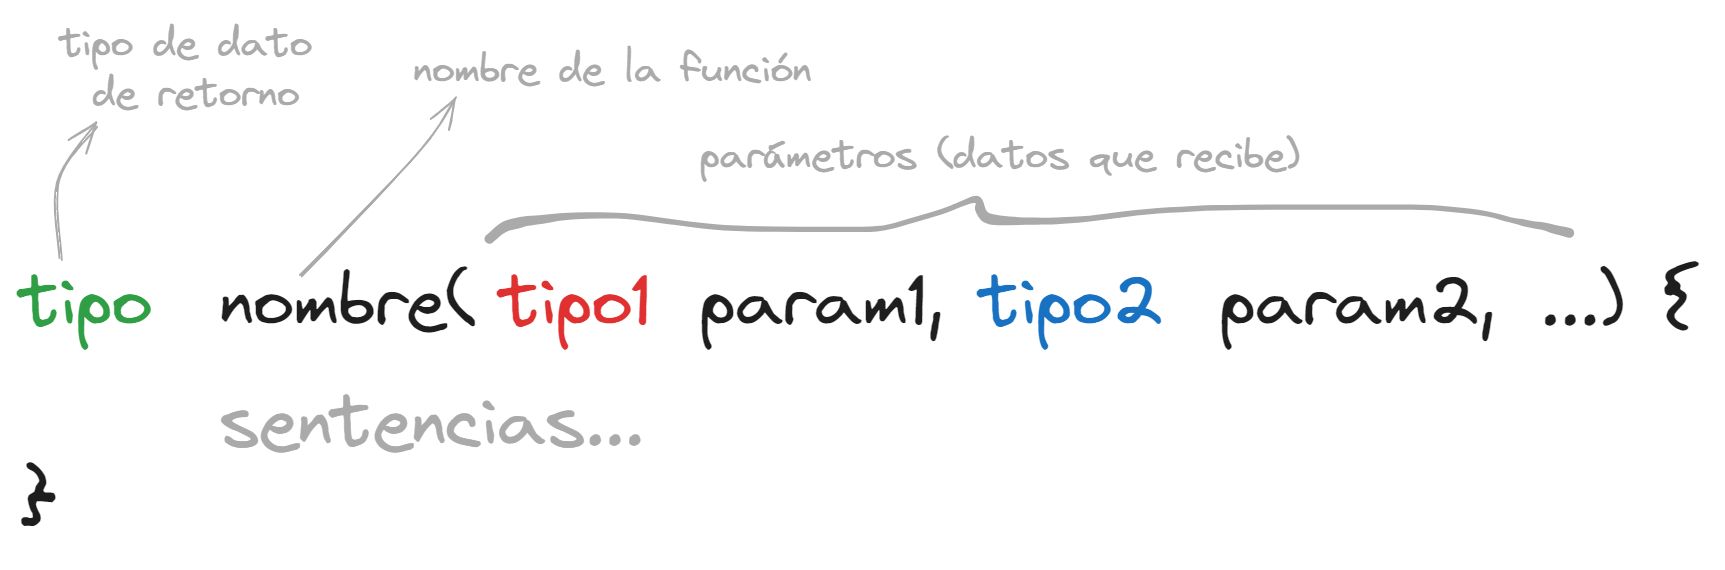
\includegraphics[width=\textwidth]{funcion.png}

\end{frame}

\begin{frame}[fragile]{Estructura de una función: ejemplos}
\begin{lstlisting}[basicstyle=\tiny]
int sumar(int a, int b, int c) {
    return a + b + c;
}

int alCuadrado(int x) {
    return x * x;
}

double distanciaEntrePuntos(double x1, double y1, double x2, double y2) {
    double restaX = x2 - x1;
    double restaY = y2 - y1;
    return sqrt(restaX*restaX + restaY*restaY);
}

void imprimirDigitos(int num) {
    while(num > 0) {
        cout << num % 10 << endl;
        num /= 10;
    }
}

int main() {
    int x = 1995;
    cout << sumar(10, x, 5) << endl; // imprime 2010

    double distancia = distanciaEntrePuntos(1, 1, 2.5, 2.5);
    cout << distancia << endl; // imprime la distancia entre (1,1) y (2.5,2.5)

    imprimirDigitos(x); // imprime 5 9 9 1
}
\end{lstlisting}
\end{frame}

\begin{frame}[fragile]{Pasaje de parámetros: por copia}
    Al momento de invocar una función, se crea una copia de los parámetros que se brindan.
    Esto significa que dentro de la función estaremos trabajando con nuevas variables. \\
\begin{lstlisting}[basicstyle=\tiny]
void imprimirTriple(int x) {
    x = 3 * x;
    cout << "3*x = " << x << endl;
}      

int main() {
    int miVar = 10;
    cout << "valor de miVar: " << miVar << endl;
    imprimirTriple(miVar);
    cout << "valor de miVar: " << miVar << endl;
    // salida:
    // valor de miVar: 10
    // 3*x = 30
    // valor de miVar: 10
}
\end{lstlisting}

En el ejemplo \alert{miVar} no se modifica, ya que al invocar la función se copia su contenido en la variable x de la función.

\end{frame}

\begin{frame}[fragile]{Pasaje de parámetros: por referencia}
    Si queremos que el contenido de \alert{miVar} se modifique, debemos definir en la función que \alert{el parámetro x pasa por referencia}.
    
    \medskip
    
    Para indicar que un parámetro pasa por referencia, debemos agregar el símbolo \alert{\&} antes del nombre del parámetro
    \begin{columns}
        \column{0.65\textwidth}\begin{lstlisting}[basicstyle=\tiny]
void imprimirTriple(int & x) {
    x = 3 * x;
    cout << "3*x = " << x << endl;
}      

int main() {
    int miVar = 10;
    cout << "valor de miVar: " << miVar << endl;
    imprimirTriple(miVar);
    cout << "valor de miVar: " << miVar << endl;
    // salida:
    // valor de miVar: 10
    // 3*x = 30
    // valor de miVar: 30
}
\end{lstlisting}
        \column{0.35\textwidth}
\includegraphics[width=\textwidth]{meme.jpg}
    \end{columns}

\end{frame}

\begin{frame}[fragile]{Pasaje de parámetros: ¿Qué se imprime?}
\begin{lstlisting}
int funcion1(int x, int & y) {
    x = y - 10;
    return y;
}

int funcion2(int & param) {
    int y = 10;
    y = funcion1(param, y);
    return y + param++;
}

int main (){
    int x = 100;
    cout << funcion2(x) << endl;
    cout << x << endl;
}

\end{lstlisting}

\end{frame}

\begin{frame}[fragile]{Funciones recursivas}
    Las funciones recursivas son aquellas que \alert{se invocan a sí mismas}. Tienen: \\
    \begin{itemize}
        \item Un conjunto de \alert{casos base}: aquellos que se utilizan para terminar con la recursión.
        \item Un conjunto de \alert{casos recursivos}: aquellos en donde se invoca a la propia función.
    \end{itemize}
    \begin{columns}
        \column{0.5\textwidth}\begin{lstlisting}[basicstyle=\tiny]
void forRecursivo(int i, int fin) {
    if (i == fin)
        return;
    
    cout << i << endl;
    forRecursivo(i+1, fin);
}

int main() {
    // imprime todos los numeros
    // entre 0 y 10
    forRecursivo(0, 10);
}
\end{lstlisting}
    \column{0.5\textwidth}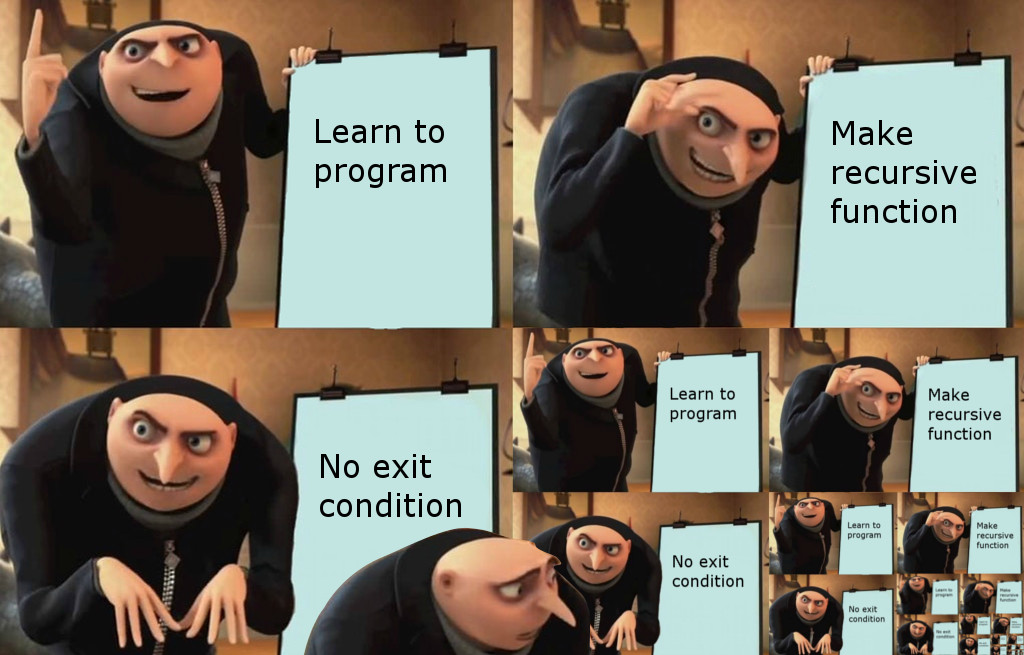
\includegraphics[width=\textwidth]{recursion.jpg}
    \end{columns}

\end{frame}

\begin{frame}{Ejercicios de funciones}
    \centering Cualquier ejercicio, todos se pueden plantear con funciones
\end{frame}


\end{document}